\documentclass[11pt,a4paper]{article}
\usepackage[utf8]{inputenc}
\usepackage[T1]{fontenc}
\usepackage{tikz}
\usepackage{amsmath,amsfonts,amssymb,amsthm}
\usepackage{graphicx}
\usepackage{mathtools}
\usepackage{exercise}
\usepackage{fullpage}


\title{TD2 MVFA:\@Linear-Time properties}
\date{}


\def\exercise#1{\Large\textbf{Exercise #1}\normalsize\\}
\def\question#1{\textbf{Question #1:}\quad}

\def\ts{\mathcal{TS}}
\def\tss{\mathcal{TS^*}}
\def\traces{\mathit{Traces}}
\def\seta{\{a\}}
\def\setab{\{a,b\}}

\newtheorem*{lemma}{Lemma}
\newtheorem*{theorem}{Theorem}
\DeclareMathOperator{\Pref}{Pref}
\DeclareMathOperator{\Cl}{Cl}

\begin{document}
\maketitle

\section*{Exercise 1}

Give the traces on the set of atomic propositions $\{a,b\}$ of the following transition system:

\begin{center}
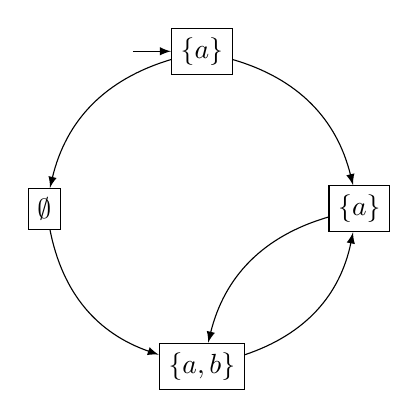
\begin{tikzpicture}
\node[draw] (s0) at (0,0) {$\emptyset$};
\node[draw] (s1) at (2,-2) {$\{a,b\}$};
\node[draw] (s2) at (2,2) {$\{a\}$};
\node[draw] (s3) at (4,0) {$\{a\}$};
\node (i) at (1,2) {};
\draw[-latex] (s0) [bend right] to (s1);	
\draw[-latex] (s1) [bend right] to (s3);
\draw[-latex] (s3) [bend right] to (s1);
\draw[-latex] (s2) [bend right] to (s0);
\draw[-latex] (s2) [bend left] to (s3);
\draw[-latex] (i) -- (s2);
\end{tikzpicture}	
\end{center}

\begin{Answer}[number=1]
Let $\ts$ be the transition system. There is only possibles executions in $\ts$, with distinct traces.
We have:
$$\traces(\ts)=\seta{(\seta\setab)}^\omega\ +\ \seta\emptyset{(\setab\seta)}^\omega$$
\end{Answer}

\section*{Exercise 2}

You have seen a way to transform a transition system $TS$ with terminal states into an ``equivalent'' transition system $TS^*$ without terminal states.

\begin{enumerate}
	\item Give a formal definition of this transformation.
	\item Prove that the transformation preserves trace-equivalence, \textit{i.e.} show that if $TS_1$ and $TS_2$ are such that $Traces(T_1) = Traces(T_2)$, then $Traces(T_1^*) = Traces(T_2^*)$.
\end{enumerate}

\begin{Answer}[number=2]
\Question%
Let $\ts=(S,\mathit{Act},\rightarrow,S_0,\mathit{AP},L)$ be a transition system.

We define another transition system without terminal states, $\tss$. Informally, it corresponds to $\ts$ without terminal states: each terminal state has been redirected to a new state which loops on itself.

$$\tss=(S\uplus\{\Omega\},\mathit{Act}\uplus\{\alpha\},\rightarrow^*,S_0,\mathit{AP},L^*)$$

In which $\Omega$ is a new state and $\alpha$ a new action.

We define $\rightarrow^*$:
$$\rightarrow^*\quad=\quad\rightarrow\quad\cup\quad\{v\xrightarrow{\alpha} \Omega~|~\nexists (s\in S, \beta\in\mathit{AP}), v\xrightarrow{\beta}s\}\quad\cup\quad\{\Omega\xrightarrow{\alpha}\Omega\}$$
Which means that every connected states in $\mathcal{TS}$ still is in $\mathcal{TS^*}$, any state with no successor is connected to $\Omega$ and $\Omega$ is connected to itself.\\

Then, we define $L^* : S\uplus\{\Omega\} \longrightarrow \mathit{AP}$ such as $\forall s\in S,  L^*(s) = L(s)$ and $L^*(\Omega) = \emptyset$. \\
\par Note that with this construction, we do not have the equivalence of trace-equivalence in $\ts$ and $\tss$, as this last adds new path ending with $\emptyset^\omega$. 
It is not necessary in our context, as we only want the first implication. If this rafinement is nevertheless wanted, it can be obtained by defining a new proposition true only in state $\Omega$.

\Question%
We introduce a lemma that will be helpful in order to prove the theorem.
\begin{lemma}
  \begin{align*}
    \traces(\tss) &= \{t\in\traces(\ts)~|~t\text{ is infinite}\}\\
    &\cup\{t\emptyset^\omega~|~t\in\traces(\ts)\text{ and $t$ is finite}\}
  \end{align*}
\end{lemma}
\begin{proof}
  By double inclusion.\\
  \begin{itemize}
  \item \reflectbox{$\subseteq$} : % explain more? -> Proof proposal
  \begin{itemize}
  \item Let $t\in \traces(\ts)$ be the infinite trace of execution $e$. As $t$ is infinite, so is $e$ (there is a state in $e$ for each subset of $AP$ in $t$). 
  Then $e$ never reach a terminal state, else it would not be infinite. So $e\in \traces(\tss)$ as $\tss$ is equal to $\ts$ out of the terminal states and $\Omega$.
  \item Let $t\in \traces(\ts)$ be a finite trace corresponding to (finite) execution $e$. Then $e$ end in a terminal state. Then,$e$ is an execution fragment over $\tss$ 
  (by construction of $\tss$ all execution fragments over $\ts$ fit $\tss$). Let $s$ be the final state ending $e$. There is no execution fragment in $\ts$ starting in $s$, 
  hence in $\tss$, only $\emptyset^\omega$ starts in $s$, corresponding to the execution $s\Omega^\omega$. The concatenation of these two fragments is possible in $\tss$ and has for trace $t\emptyset^\omega$.
  \end{itemize}
  \item $\subseteq$ : Here it is easier to work directly with the underlying execution. 
  Let $t\in \traces(\tss)$ be the trace of execution $e$. Let us discuss on the reach of $\Omega$.
  \begin{itemize}
  \item If $e$ reaches $\Omega$ at some point, then as $Post(\Omega) = \{\Omega\}$, $e=e'\Omega^\omega$ where $e'$ is a finite (and initial) execution fragment without $\Omega$ over $\tss$. 
  So $e'$ is an initial finite execution fragment over $\ts$. Furthermore the last state $s$ of $e$ is such that $\Omega \in Post(s_{\tss})$, so by construction of $\tss$ $Post(s_{\tss})=\Omega$ and 
  $Post(s_{\ts})=\emptyset$. Hence $e'$ is maximal, i.e. $e'$ is a finite execution of $\ts$ of trace $t'$. By construction of $e$ and $t$ (the initial trace over $\tss$), $t = t'\emptyset^\omega$.
  \item If $e$ does not reach $\Omega$, then $e$ is an infinite execution over $\ts$ and $t\in  \{t\in\traces(\ts)~|~t\text{ is infinite}\}$.
  \end{itemize}
  \end{itemize}
\end{proof}


\paragraph{Trace-equivalence preservation:} Let $\ts_1$ and $\ts_2$ be two transition systems such that $\traces(\ts_1)=\traces(\ts_2)$. Let $t_1\in\traces(\tss_1)$. Let us show that $t_1\in\traces(\tss_2)$.

According to the previous lemma, $t_1$ can either be in $\{t\in\traces(\ts_1)~|~t\text{ is infinite}\}$ or in $\{t\ \emptyset^\omega~|~t\in\traces(\ts_1)\text{ and $t$ is finite}\}$.

If $t_1\in\{t\in\traces(\ts_1)~|~t\text{ is infinite}\}$, then $t_1\in\traces(\ts_1)=\traces(\ts_2)$. Thus, $t_1$ is an infinite trace of $\ts_2$ and then by the previous lemma, $t_1\in\traces(\tss_2)$.

If $t_1\in\{t\ \emptyset^\omega~|~t\in\traces(\ts_1)\text{ and $t$ is finite}\}$, then $t_1=t\ \emptyset^\omega$ where $t$ is a finite trace of $\ts_1$ and thus a finite trace of $\ts_2$ as well. Then by the previous lemma, $t\ \emptyset^\omega$ is also a trace of $\tss_2$.

We thus have that every trace of $\tss_1$ is a trace of $\tss_2$, which means $\traces(\tss_1)\subseteq\traces(\tss_2)$. The other inclusion is symmetric. We thus have proved that, whenever $\traces(\ts_1)=\traces(\ts_2)$, $\traces(\tss_1)=\traces(\tss_2)$.\\
\end{Answer}

\section*{Exercise 3}

\def\badp{\mathit{BadPref}}
\def\pref{\mathit{Pref}}
\def\twoap{2^{AP}}
\def\star{^*}

Consider the set $AP$ of atomic propositions defined by $AP = \{ x = 0,x > 0 \}$ and consider a non-terminating sequential computer program $P$ that manipulates the variable $x$.

Formulate the following informally stated properties as LT properties:
\begin{enumerate}
\item false;
\item initially $x$ is equal to zero;
\item initially $x$ differs from zero;
\item initially $x$ is equal to zero, but at some point $x$ exceeds zero;
\item $x$ exceeds zero only finitely many times;
\item $x$ exceeds zero infinitely often;
\item the value of $x$ alternates between zero and not zero;
\item true.
\end{enumerate}

Determine which of the provided LT properties are
safety properties and which are liveness properties. 

\begin{Answer}[number=3]
  \Question 
Every prefix is a bad prefix for the propery \textit{false}, because the property is always false. Thus, $\badp(false) = (\twoap)\star$ and $\pref{false} = \emptyset$. As $\pref(false)\neq (\twoap)\star$, the property is not a liveness property. However, the property is a safety property because for each infinite word, there exists a finite prefix that cannot be extended into an accepted word : any prefix of the infite word is such a prefix.
  \Question
For such a property, one can define a set of bad prefixes : $\badp = \{x > 0\}(\twoap)\star$. Any infinite word that make the property false has such a bad prefix. Thus, the property is a safety property. However, since $\badp\neq\emptyset$, there exists some finite words that cannot be extended into an accepted infinite word. Thus, the property is not a liveness property.
  \Question%
  \Question%
  \Question%
  \Question%
  \Question%
  \Question%
\end{Answer}

\section*{Exercise 4}
Let $P$ and $P'$ be two LT properties. Prove or disprove: $Pref(P) = Pref(P')$ if and only if $Cl(P) = Cl(P')$.

\begin{Answer}[number=4]
  Let $P$ and $P'$ be two LT properties. The following theorem is true:
  \begin{theorem}
    $\Pref(P) = \Pref(P')$ if and only if $\Cl(P) = \Cl(P')$
  \end{theorem}
  \begin{proof}
    We prove the two implications.
    \begin{description}
      \item[($\Rightarrow$)]
        Suppose $\Pref(P) = \Pref(P')$. We have:
        \begin{align*}
          \Cl(P) &= \{\sigma\in{(2^{\textrm{AP}})}^\omega \mid \Pref(\sigma)\subseteq\Pref(P)\}\\
          &= \{\sigma\in{(2^{\textrm{AP}})}^\omega \mid \Pref(\sigma)\subseteq\Pref(P')\} &&\text{ since }\Pref(P) = \Pref(P')\\
          &= \Cl(P')&&\text{ (definition of closure)}
        \end{align*}
      \item[($\Leftarrow$)]
        Suppose $\Cl(P) = \Cl(P')$. We have two cases:
        \begin{description}
          \item[Case 1] One of $\Pref(P)$ or $\Pref(P')$ is empty.\\
          Suppose for example that $\Pref(P) = \emptyset$ Then $\Cl(P) = \emptyset = \Cl(P')$.\\
          Thus $\Pref(P') = \emptyset = \Pref(P)$.
          \item[Case 2] $\Pref(P) \neq \emptyset$
          Let $\sigma\in\Pref(P)$ be a prefix of $P$. \\
          There exists an (infinite) trace $\hat{\sigma} \in P$ such that $\sigma\in\Pref(\hat{\sigma})$.

          Since $\hat{\sigma}\in P\subset\Cl(P)$, we have that $\hat{\sigma}\in\Cl(P')$. \\
          Therefore $\sigma\in\Pref(P')$.\\
          $\Pref(P)\subseteq\Pref(P')$. The other inclusion is true for the same reason.

        \end{description}
    \end{description}
  \end{proof}
\end{Answer}

\section*{Exercise 5}
Let $P$ and $P'$ be liveness properties over $AP$. Prove or disprove the following claims:
\begin{enumerate}
\item $P \cup P'$ is a liveness property;
\item $P \cap P'$ is a liveness property.
\end{enumerate}
Answer the same questions for $P$ and $P'$ being safety properties.

\begin{Answer}[number=5]
\Question%
Let us prove that for $P$ and $P'$ two liveness properties, $P \cup P'$ is a liveness property. 
\begin{align*}Pref(P \cup P') &= Pref(P) \cup Pref(P')\footnotemark[1]\\ 
                              &= (2^{AP})^* \cup (2^{AP})^* \text{ [P and P' are liveness properties]}\\ 
                              &= (2^{AP})^*
\end{align*}
So $P \cup P'$ is a liveness property.
\footnotetext[1]{If this equality is not known, we can convince ourselves by considering that being a prefix of a language by definition being a prefix of a given word, 
and the words of $A\cup B$ are exactly the words of $A$ plus the words of $B$.}
\Question%
Let us show a counterexample proving that the intersetion of two liveness properties is not always a liveness property.
Using the two liveness properties defined in exercice 3: $x$ exceeds zero only finitely many times; $x$ exceeds zero infinitely often.
The intersection of these two properties is $false$ which is not a liveness property (cf. exercice 3 again).
\Question%
Given $P$ and $P'$ two safety properties, we prove that $P\cup P'$ is a safety property, by reasoning on the bad prefixes. We show by double inclusion that $ not( P\cup P') = BadPref( P\cup P')$
\begin{itemize} 
\item $\alpha \notin P\cup P'$ implies $\alpha \notin P$ or $\alpha \notin P'$. 
For the simplicity of the notations, we will assume $\alpha \notin P$ is verified. Then $\alpha \in BadPref(P)$, i.e. $Pref(\alpha) \subseteq Pref(P) subseteq Pref(P \cup P')$ and $\alpha \in BadPref(P \cup P')$.
\item $alpha \in BadPref(P\cup P')$ means $Pref(\alpha) \subseteq Pref(P \cup P')$ which implies $alpha \in BadPref(P)$ (or the same thing for $P'$, an the proof is symmetric). Then, by def $\alpha \in P \subseteq (P \cup P')$.
\end{itemize}
\Question%
Given $P$ and $P'$ two safety properties, we prove that $P\cap P'$ is a safety property, by showing the equality of this language with its cloture.
As for any property $p$, $p \subseteq \Cl(p)$, we will prove the other inclusion. Lets consider $\alpha \in \Cl(P\cap P')$. By definition, $Pref(\alpha) \subseteq Pref(P\cap P') \subseteq Pref(P) \cap Pref(P')$\footnotemark[2].
Specificly, $Pref(\alpha) \subseteq Pref(P)$, hence $\alpha \in \Cl(P) = P$. The same proof leads to $\alpha \in P'$. Hence $\alpha \in P\cap P'$.


\footnotetext[2]{As previously, if this is not known, convince yourself with this argument: being a prefix of $A\cap B$ is being the prefix of a word of $A \cap B$ wich is a word of both $A$ and $B$.}
\end{Answer}


\end{document}
